% !TEX root = ../main.tex

\chapter{Aspirations}
\label{ch:future}

\startcontents[chapters]

\vfill

\begin{alltt}\sffamily
Mid the silence that pants for breath,
when I thought myself at my last gasp,
haine ou de l'ambition et qui se,
the pale motor vessel withdrew its blue breath toward the island's horizon.

As pure and simple as a powder puff,
such also was the ambition of others upon the like occasion,
there was hardly a breath of air stirring,
mon ancien cœur en une aspiration vers la vertu.

After drawing a long breath,
the silver ring she pull'd,
the suitor cried, or force shall drag thee hence.

For wild ambition wings their bold desire,
and with thine agony sobbed out my breath,
I will pull down my barns.
\end{alltt}

\newpage
\minicontents
\spirals


Developing a software product rarely finishes. It is maintained, refactored, repurposed, updated, extended, etc. Especially with creative products, where the functional requirements are more fluid perhaps, it is always tempting to change things. 

For the purpose of this doctoral project, the artefact \url{pata.physics.wtf} is a snapshot of a product in constant motion. The state of the code at the time of submission of this thesis is described in chapter~\ref{ch:implementation}\marginpar{§~\ref{ch:implementation}} and further elaborated on in the \nameref{ch:analysis} chapter\marginpar{§~\ref{ch:analysis}}. But it may very well continue to evolve.

Here, in this chapter I will lay out some of the potential further work for this project. This may continue on a private basis or in a more academic environment. 


\section{Performance}
\label{s:performance}

\paragraph{Startup} 
The website can be slow to load. Currently speed performance was not a priority during development. In fact it is not built for speed from the ground up. Each time the server restarts, the indexing process takes place from scratch (see chapter~\ref{s:setup}\marginpar{§~\ref{s:setup}}). This takes time. Google and other big web search engines do this continuously in the background to keep data up to date. The index\marginpar{§~\ref{s:index}} is currently cached after startup but perhaps preprocessing it and storing it more permanently in a database would help speed up the start. However this may not be necessary, as it only affects the server startup.

\paragraph{Query Response} 
The time it takes from the user entering a query term and the system displaying the results page varies between unnoticable short and impatiently long. This is due to the pataphysicalisation process. This requires calls to external and internal \ac{API}s such as Flickr and WordNet. See analysis on speed issues in table~\ref{tab:percent}\marginpar{\faicon{table}~\ref{tab:percent}}.

\paragraph{Preprocessing Corpora} 
At this point the texts in the corpora consist of almost unedited plaintext (`.txt') files\footnote{For text files downloaded from Project Gutenberg, the Gutenberg specifc copyright notices have been removed to only contain the relevant body of text.} (see chapter~\ref{s:corpora}\marginpar{§~\ref{s:corpora}}). Newlines and whitespace formatting varies, as does language and quality of spelling. Generally, chapter headings, chapter numberings, etc. were left untouched. The Shakespeare corpus contains poetry and plays for example. With the plays, scene information, stage directions, and voice details were kept. This means sentences that appear in the results of the search tool can contain peripheral words such as in this example: ``\ldots Athens and a wood near it ACT I \ldots'' from \textit{A Midsummer Night's Dream} or this example: ``\ldots Exit SHERIFF Our abbeys and our priories shall pay This expedition's charge \ldots'' from \textit{King John}. This could be addressed by preprocessing the individual texts in advance and removing any text that might interfere with the readablility of results.

\paragraph{Image Sizes} 
At the moment images are retrieved at one specified size through the various \ac{API} calls even though they are displayed at various different sizes depending on their location in the image spiral (unless they are displayed as a list). This process could certainly be optimised. Smaller image sizes could be accessed via the \ac{API}s.


\section{Design}
\label{s:designaspi}

\paragraph{Responsive Spirals} 
Currently the image and video spirals (see chapter~\ref{s:imgvid}\marginpar{§~\ref{s:imgvid}}) are fixed size. This means that when the webpage is resized the spiral stays the same size and is left-aligned on the page. Ideally it would be better to scale the spiral with the width of the browser page. This could be achieved using percentage widths, although it would require a lot of work to adapt the current code for the spirals (see chapter~\ref{s:imgspiral}\marginpar{§~\ref{s:imgspiral}}).

\paragraph{Scalable Image Sizes} 
As mentioned above, images are retrieved at one size through the various \ac{API} calls. Because images in the spiral have different sizes according to where in the spiral they are located, they are scaled up or down directly in the \ac{HTML} code. This means that some of the images look distorted and pixelated if they have to be scaled up or down too much.

\paragraph{Square Aspect Ratio} 
Another issue is the aspect ratio of images and videos. For the spiral they need to be square. They are currently distorted as opposed to cropped. It might be possible to specify an option in the \ac{API} calls to only retrieve square images which would help this problem.

\paragraph{Responsive Poems} 
A similar problem to the responsive spirals exists with the display of the Queneau poems. The random poems are centered on the page but the Queneau poems require a lot more formatting and styling to render and currently this is achieved by left-aligning them and having a fixed `absolute' position on the page. Ideally this would also be centered as in the random poems. 

\paragraph{Paginate Results}
For the text-by-source and text-by-algorithm search as well as the image- or video-as-list search results, it may improve the loading speed of the results page to split the results into smaller chunks and display them on several pages instead of one long scrolling page. This is called pagination.

\paragraph{Random Sentences} 
Adding to the source of random sentences used in the top and bottom banner on the website should be an ongoing endeavour. The current list of sentences used is shown in appendix~\ref{s:appsentences}\marginpar{§~\ref{s:appsentences}}.


\section{Text}
\label{s:textfuture}

\paragraph{Result Sentences} 
Currently the way result sentences are retrieved for the text search is based on punctuation (see chapter~\ref{s:ressent}\marginpar{§~\ref{s:ressent}}). This means once a pataphysicalised keyword has been found, the system retrieves up to \num{10} words prior until it reaches a punctuation mark and the same for after. The idea here was to get suitable sentence fragments. This could be changed to rely on \ac{POS} tags for example or simply retrieving complete sentences.

\paragraph{Stopwords}
When the index is created only words that are not considered stopwords are added. We could modify the list of stopwords (see appendix~\ref{s:stopwords}\marginpar{§~\ref{s:stopwords}}) to include a few more uninteresting words. Or we could simply remove everything but nouns for example. This would drastically influence the results produced by the system.

\paragraph{Rhyming Scheme} 
One of the biggest points for future work is to introduce a rhyming scheme for the poetry results. This might involve some more \ac{NLP} during the creation of the index\marginpar{§~\ref{s:index}}. It would make the poems much more readable. This could include pronounciation \ac{POS} tags or other \ac{IPA} like data (for example using an \ac{API} like Wordnik \autocite{Wordnik2016} or a library like \ac{NLTK}). So a word in the index dictionary might contain the following items.

\begin{minted}{text}
  (``tree'': [``l_00'': [24,566,4990], ``s_14'': [234,5943]], ``[tri]'')
\end{minted}

By doing \ac{POS} tagging\marginpar{§~\ref{s:pos}} with pronounciation data, we could retrieve sentences that match the sound of the last word of the previous line for example.


\section{Pataphysicalisation}
\label{s:pataasp}

\paragraph{WordNet}
The vocabulary in WordNet is limited. According to its website \autocite{Princeton2010} it contains \num{117000} `synsets'\footnote{Synonyms---``words that denote the same concept and are interchangeable in many contexts''---are grouped into unordered sets called synsets \autocite{Princeton2010}.} This affects two of my algorithms (namely the Syzygy and Antinomy algorithms). See also discussion in chapter~\ref{s:analsyzygy}\marginpar{§~\ref{s:analsyzygy}}. An option might be to somehow widen the amount of word matches by including different word-types/forms and relationships, such as troponyms, homonyms and heteronyms. Using these could introduce a whole new kind of pataphysical result. 

Homonyms are pronounced the same but mean something else (e.g. `write' and `right'). Heteronyms are words that are spelled the same but have a different meaning (e.g. `close to the edge' and `to close the door'). Homophones are often used to create puns (and remember---puns are syzygys of words), for example ``past your eyes'' and ``pasteurize''. 

\begin{quotation}
   You can tune a guitar, but you can't tuna fish. Unless of course, you play bass. \sourceatright{(attributed to Douglas Adams)}
\end{quotation}

\paragraph{Antinomy}
The antinomy algorithms relies on WordNet's antonyms. A lot of words simply do not have an opposite and no fallback is currently defined. This means a lot of the time the antinomy function will not produce any results. Andrew Dennis implemented the algorithm in the same way, as discussed in chapter~\ref{s:dennis}\marginpar{§~\ref{s:dennis}}. It would be great to come up with a better way of dealing with this concept to ensure results are produced everytime.

\paragraph{Stemming}
Stemming could increase the number of results found by all algorithms (see chapter~\ref{s:nlp}\marginpar{§~\ref{s:nlp}}). A danger of increasing the output of the pataphysicalisation is always that results become more boring. Currently queries such as `clear' and `clearing' are treated as separate entities and would produce different results. Stemming would turn both of these words into the stem `clear' and they would return the same results. Now it becomes immediatly clear (no pun intended) though that this might not always be desirable as just illustrated in this sentence: the root meaning of `clear' can be very different to the meaning of `clearing'.

\paragraph{Queneau's poems}
It would be nice to actually add Queneau's poems \autocite{Queneau1961} into the Faustroll corpus as little easter egg (see chapter~\ref{s:culture}\marginpar{§~\ref{s:culture}}).

\paragraph{Image Algorithms}
The image and video search currently rely on external \ac{API}s (see chapter~\ref{s:imgvid}\marginpar{§~\ref{s:imgvid}}). One option to approach this in a totally different way would be to write algorithms that analyse and pataphysicalise the actual image or video data themselves. This might involve manipulating histograms or pixel maps.

\paragraph{Maximum Obscurity}
N-grams are a \ac{NLP} technique introduced in chapter~\ref{s:ngrams}\marginpar{§~\ref{s:ngrams}}. The idea is that it allows for prediction of likely word pairs, meaning if the word `sunny' often occurs just before the word `day' in a given training text or corpus then the probability for this particular n-gram is higher than say for `sunny dog'. This can be increased to predict the probability of longer chains of words. One can immediately see the attraction of abusing this to generate pseudo sentences or even of creating a formula similar in nature but for example ranking obscure combinations of words higher than common ones. So for example instead of having a \acf{MLE} (see equation~\ref{eq:mle}\marginpar{$\bm{\Sigma}$~\ref{eq:mle}}) we could have a `Maximum Obscurity Estimation' which returns the highest probabilty for word sequences that happen the rarest.

\paragraph{Pataphysical Entropy}
Similarly, we could play with maximum entropy models as shown in chapter~\ref{s:maxent}\marginpar{§~\ref{s:maxent}} together with \ac{POS} tagging\marginpar{§~\ref{s:pos}} by rigging given probability for tags. There are endless possibilities of abusing these kinds of techniques. This is also very reminiscent of \ac{OULIPO} techniques. 

\paragraph{Grammars}
We could create a whole new language grammar based on pataphysical principles. Examples of using a standard grammar (see chapter~\ref{s:grammars}\marginpar{§~\ref{s:grammars}}) for generating `random' text are as follows\footnote{\autocite{Winter2016,Dada2016,Stribling2016}}.

\begin{adjustwidth}{1cm}{}
\begin{description}[leftmargin=3cm]
  \item[ArtyBollocks] Generates artist statements.
  \item[DadaEngine] A system for generating random text from grammars.
  \item[SciGen] Generates random Computer Science research papers.
\end{description}
\end{adjustwidth}

\paragraph{Uncreativity}
In chapter~\ref{s:csf}\marginpar{§~\ref{s:csf}} I discussed the concepts of uninspiration and aberration by Wiggins and Ritchie \autocite*{Wiggins2006,Ritchie2012} in relation to their \ac{CSF}. We could define a `Pataphysical Search Framework' in the same way. Table~\ref{tab:csf}\marginpar{\faicon{table}~\ref{tab:csf}} shows some of their original definitions for various forms of aberration and uninspiration. Table~\ref{tab:patacsf}\marginpar{\faicon{table}~\ref{tab:patacsf}} then shows some rough ideas about how pataphysical concepts might be defined.

\begin{adjustwidth}{1cm}{}
\begin{description}[leftmargin=2.5cm]
  \item[Clinamen] smallest possible aberration to make the biggest difference
  \item[Antimomy] reachable, abnormal concepts with value
  \item[Anomaly] reachable concepts outside the norm
  \item[Absolute] criteria for value and norm must be perfectly matched
  \item[Syzygy 1] concepts reachable within 3 steps from the query
  \item[Syzygy 2] transformed set of concepts $S_{obj} \rightarrow S^{meta} \rightarrow S'{obj}$
\end{description}
\end{adjustwidth}

This is definitely work in progress and it would be out of the scope of this thesis to elaborate much further.

\begin{table}[!htbp]
\centering
\caption{CSF concept definitions of uncreativity (see chapter~\ref{s:csf})}
\label{tab:csf}
\begin{tabu}{ll}
\toprule
\textbf{Name} & \textbf{Equation} \\
\midrule
Universal set of concepts & $U$ and $X \subseteq U$ \\
Aberration & $B \text{ where } B \notin N_\alpha (X) \ \wedge \ B \neq \emptyset$ \\
Perfect Aberration & $V_\alpha (B) = B$ \\
Productive Aberration & $V_\alpha(B) \neq \emptyset \ \wedge \ \neq B$ \\
Pointless Aberration & $V_\alpha(B) = \emptyset$ \\
Hopeless Uninspiration & $V_\alpha (X) = \emptyset$ \\
Conceptual Uninspiration  & $V_\alpha (N_\alpha (X)) = \emptyset$ \\
Generative Uninspiration  & $elements(A) = \emptyset$ \\
\bottomrule
\end{tabu}
\end{table}

\begin{table}[!htbp]
\centering
\caption[CSF pataphysical concepts]{Possible definitions of pataphysical concepts in terms of the CSF}
\label{tab:patacsf}
\begin{tabu}{XX[5]} 
\toprule
\textbf{Name} & \textbf{Equation} \\
\midrule
Norm & $N_\alpha (X) = \{c \in X \ | \ N(c)> \alpha\} \text{ where } N \in [0,1]^X$ \\
Value & $V_\alpha(X) = \{c \in X \ | \ V(c) > \alpha\} \text{ where } V \in [0,1]^X$ \\
Pata & $P_\alpha(X) = $ \newline $\{c \ | \ c \in(CLI(X)\cup ANT_\alpha(X) \cup SYZ(X) \cup ANO_\alpha(X) \cup ABS(X))\}$ \\
Clinamen & $CLI(X) = \{c \in X \ | \ N_{0.9} (N_{0.1} (c))\}$ \\
Antinomy & $ANT_\alpha(X) = \{c \in X \ | \ V(N_0(c)) > \alpha\}$ \\
Anomaly & $ANO_\alpha(X) = \{c \in X \ | \ N(c)< \alpha\}$ \\
Absolute & $ABS(X) = \{c \in X \ | \ V_1 (N_1 (X)) \neq \emptyset\}$ \\
Syzygy 1 & $SYZ(query) = \bigcup_{n=0}^{3} elements(Q(N,V)^n (query))$ \\
Syzygy 2 & $SYZ(X) = S'(X) \text{ where } S_{obj} \rightarrow S^{meta} \rightarrow S'{obj}$ \\
\bottomrule
\end{tabu}
\end{table}


\section{Extensions}
\label{s:extensions}

\paragraph{Additional APIs} 
Currently 5 \ac{API}s\footnote{Flickr, Getty, Bing, MicrosoftTranslator and YouTube} are used in \url{pata.physics.wtf}. This could be increased to include more varied sources of data. Sites like Flickr are heavily based on user tags (`folksonomies') which can be unreliable and a bit random at times. Possible additional \ac{API}s to consider would be Instagram, Imgur, Facebook, Google Image Search, DeviantArt, Pinterest, Vimeo, Twitter, SoundCloud, etc.

\paragraph{Web Search} 
The use of \ac{API}s could also include web search results rather than just images and videos. This would need its own interface section and a suitable display style for the results. The biggest problem for this are \ac{API} limitations as mentioned in chapter~\ref{s:apis}\marginpar{§~\ref{s:apis}}. Alternatively a ready-made index or crawl could be used but these are typically many terrabytes in size and have a cost attached. Crawling the web myself is not an option due to the computational power, time and space required to do so.

\paragraph{Additional Algorithms} 
It would be nice to implement some more algorithms for the search tool. This could include the two additional algorithms suggested by Andrew Dennis (see chapter~\ref{s:dennis}\marginpar{§~\ref{s:dennis}}) or developing more of my own. This could involve implementing some of the other pataphysical principles, such as equivalence or anomaly. Or it could consist of implementing some of the more famous \ac{OULIPO} techniques. The repertoire of them is huge (see tables~\ref{tab:oulipo1} and \ref{tab:oulipo2}\marginpar{\faicon{table}~\ref{tab:oulipo1} \& \ref{tab:oulipo2}}).

\paragraph{Custom API}
Finally, it would be great to develop a custom \ac{API} for the algorithms of \url{pata.physics.wtf}. This would allow other people to use the search remotely without going through the interface and to use the results as they want. This would have been beneficial for the Digital Opera project\marginpar{§~\ref{s:opera}} and certainly for other researchers/developers like Andrew Dennis\marginpar{§~\ref{s:dennis}}.


\section{User Testing}

\paragraph{Focus Group}
It might be interesting to look at opinions of various people (general public and experts) about the interpretation/evaluation framework. This could be done by asking them to provide their own definition of computer creativity and then to analyse and evaluate a product (such as \url{pata.physics.wtf}) according to their own criteria. Then follow this up by getting the same people to use my proposed framework\marginpar{§~\ref{s:framework}} to compare the results. This would include asking them about whether or not they thought that using the framework was beneficial to them or confusing.

\paragraph{Eye-Tracking}
To study the effects of using different styles of presenting the same results, an eye-tracking experiment could be done. This would involve setting up participants with the necessary equipment and then introduce them to \url{pata.physics.wtf} and moniter their eye movements as they navigate the site. This could also provide details about how long users spend on each results page, what kind of style of results they prefer, etc. Some may prefer image or video search over the text search while others may not be interested in that at all. Generally of course one has to take into account that this is a creative piece of work and not everybody will like it. It is purposefully purposeless and highly subjective, so user feedback may not provide unbiased and useful results.


\section{Audio}
\label{s:audio}

Audio search completes the spectrum of pataphysical search tools. Being outside the scope of this doctoral project, it is left open for potential future work, but I want to elaborate a little bit on the significant connection between pataphysics, creativity and music.

Andrew Hugill says ``pataphysics has become a byword for experimentation and left-of-field work'' in digital and electronic music \autocite*{Hugill2012}. He lists several artists \footnote{Experimental German electronica band \textit{Farmer’s Manual}, Paul D. Miller, better known as \textit{DJ Spooky}, American ambient experimental musician \textit{Faustroll}, Australian-Sri Lankan rapper \textit{Pataphysics}, and electronic music artist \textit{Tomoroh Hidari} a.k.a. Oliver Stummer.} as examples of pataphysical musicians but highlights a few names in particular as key figures in this genre. 

\paragraph{John Cage}
John Cage was an American composer, musician, writer, philosopher, and artist (1912---1992). He is often associated with the avant-garde movement (his close friend Marcel Duchamp is also famous for his involvment in this), which itself can be said to be related to Dada, \ac{OULIPO}, and of course Pataphysics (see \autocite{Hugill2012}). Pataphysical influences abound in Cage's work and words (although he appears to be an unconscious rather than conscious Pataphysician). For example he explained he ``was shocked at college to see one hundred of my classmates in the library all reading copies of the same book. Instead of doing as they did, I went into the stacks and read the first book written by an author whose name began with Z'' \autocite{Cage1989}, an act of antinomy. A very Oulipian approach to composition comes from his use of chance: he developed ``complicated composing means using I Ching chance operations, making my responsibility that of asking questions instead of making choices'', in fact he said his work ``became an exploration of non‑intention'' \autocite*{Cage1989}. This also resembles the chance swerve of the clinamen in pataphysics.

\begin{quotation}
[\ldots] all of the incidents were critical, all of the people influenced me, everything that happened and that is still happening influences me. \sourceatright{\autocite{Cage1989}}
\end{quotation}

Cage was also influenced by Zen Buddhism, which he called a mixture of ``humor, intransigence, and detachment''\footnote{He also refers to his friend Duchamp here: ``[Zen] makes me think of Marcel Duchamp, though for him we would have to add the erotic''.} \autocite*{Cage1989}.

The antinomy and \ac{OULIPO} influences are strongest in Cage's famous \textit{4'33''} piece from 1952. Hugill compares this to an earlier, similar work by Alphonse Allais from 1884 called ``Marche funèbre composée pour les funérailles d’un grand homme sourd'' (Funeral March for the Obsequies of a Large Deaf Man) \autocite*{Hugill2012}. \textit{4'33''} was inspired by Robert Rauschenberg's white paintings: ``in the anechoic chamber at Harvard University [I] heard that silence was not the absence of sound but was the unintended operation of my nervous system and the circulation of my blood'' \autocite{Cage1989}. Cage called the composition his `silent piece' and it consist of three movements, during which performers are instructed to \emph{not} play their instruments.






iPhone app:
\url{http://johncage.org/4_33.html}

\paragraph{The Beatles}
``The tip of the pataphysical iceberg in popular music may be found in The Beatles’ song “Maxwell’s Silver Hammer,” which contains probably the best-known reference to an obscure avant-garde French literary concept in the whole of music (The Beatles 1969):

  Joan was quizzical
  studied pataphysical
  science in the home.

Barry Miles recounts that Paul McCartney’s interest in pataphysics began when he heard a radio broadcast of Jarry’s play Ubu cocu (Ubu Cuckolded) on the BBC Third Programme in 1966. Paul said: “It was the best radio play I had ever heard in my life, and the best production, and Ubu was so brilliantly played. It was just a sensation. That was one of the big things of the period for me” (Miles 1997, 229).

“Maxwell’s Silver Hammer” seems to be modeled on the “Chanson du décervelage” (Debraining song) from Ubu cocu. The schoolboy Maxwell Edison’s silver hammer repeatedly comes down “bang, bang” upon the heads of those who, in their normality, have offended him in various ways, and “makes sure that they are dead.” Just like the “Chanson du décervelage,” the Beatles’ tune is reminiscent of music-hall: childishly simple and ironically joyous.

John Lennon’s politics and Paul McCartney’s interest in pataphysics combined in a way which typified their entire collaboration. As Paul commented, referring to John’s involvement with avant-gardism: “That was the big difference between me and John: whereas John shouted it from the rooftops, I often just whispered it in the drawing room, thinking that was enough” (Miles 1997, 230).

Paul’s interest in pataphysics, or at least Ubu, has continued, and in 1995 he produced a six-part radio show entitled Oobu Joobu, which aired on the American network Westwood One.''
\autocite*{Hugill2012}

\paragraph{Frank Zappa}
``The major figure, at least in spirit, was Frank Zappa, most of whose recorded output may be viewed as a pataphysical legacy, albeit not explicitly labeled as such. Zappa seems to have picked up on the interest in pataphysics generated on the West Coast by the celebrated issue 13 of the Evergreen Review, published in 1960, Roger Shattuck’s The Banquet Years, and the En glish translations of Jarry, who was seen as a precursor of figures such as William Burroughs and Hunter S. Thompson. This became part of the Zeitgeist of hippiedom and a byword for all that was “far out” or zany, a tradition that continues to this day.''\autocite*{Hugill2012}

\paragraph{Captain Beefheart}
``Bands such as The Residents and musicians such as Captain Beefheart were clearly aware of pataphysics and worked it into their output, but in a freewheeling sort of way that was inspired more by its spirit of nonconformity than by the letter of the written words.''\autocite*{Hugill2012}

\paragraph{Helge Schneider}
One of German comedian, jazz musician and multi-instrumentalist Helge Schneider's biggest hits was a song about cat litter boxes. 
``Sinn im Unsinn'' (sense in nonsense) \autocite{}
\url{https://de.wikipedia.org/wiki/Helge_Schneider}
\url{http://www.helge-schneider.de/home}

\paragraph{Andrew Hugill}
andrew hugill
\url{http://www.worldcat.org/title/pataphysical-piano-the-sound-and-silences-of-andrew-hugill/oclc/436443718}
\url{http://andrewhugill.com/compositions.html}
\url{https://soundcloud.com/andrew-hugill/catalogue-de-grenouilles}

\paragraph{Pip Greasley}
5K PURSUIT OPERA (1992)  
Acclaimed TV opera. Sport interacts with art through digital score. Channel 4 Television
\url{http://www.dmu.ac.uk/about-dmu/academic-staff/art-design-humanities/pip-greasley/pip-greasley.aspx}
\url{https://youtu.be/lo-k8JcPgKY}

\spirals

Gavin Bryars 

\paragraph{Gavin Bryars}
``In 1972, Gavin Bryars composed The Sinking of the Titanic, which explicitly set out to give a pataphysical account of the tragedy. The piece included fragments of interviews with a survivor, Morse signals played on woodblocks, references to the different bagpipe players on the ship (one Irish, one Scottish), miscellaneous sound effects relating to descriptions given by survivors of the sound of the iceberg’s impact, and other “found materials.” The “imaginary solution” that provided the most overtly pataphysical aspect of the piece, however, was the prolongation of the hymn tune “Autumn” that was famously played by the ship’s band, recorded underwater. In Bryars’s version, the band plays for eternity:

Bryars has continued to make both overt and covert references to pataphysics in his work. Many of the early experimental pieces are conceptual in nature, pieces that exist in the imagination as much as in reality. Concert works of the period also show the pataphysical presence, so Ponukélian Melody (1975), for example, is directly inspired by Roussel’s Impressions of Africa. Such ideas remain as programmatic themes in the more recent pieces.''\autocite*{Hugill2012}


\paragraph{John White}
``The veteran maverick John White continues to produce pataphysical music, most recently for the London Institute of Pataphysics, of which he has become something of a composer in residence. White’s output is vast, extending to nearly 200 piano sonatas, over 20 symphonies, more than 30 ballet scores, a body of electronic music, and a very large amount of incidental music for the stage. It is generally characterized by the kind of ironical humor and references to found material that typify a certain kind of pataphysical art. One recent work, a homage to Jacques Prévert which processes the sounds of a poem through various electronic devices, sums up the approach by being both strangely evocative and yet apparently meaningless.''\autocite*{Hugill2012}



\paragraph{Hawkwind}
``Another prog-rock band that picked up pataphysics was Hawkwind, who included the science fiction writer Michael Moorcock as an honorary member.''\autocite*{Hugill2012}

\paragraph{Sergeant Pepper’s Lonely Hearts Club Band}
``Meanwhile, Sergeant Pepper’s Lonely Hearts Club Band (1967) offered a pataphysical solution to the problem of fame. An imaginary band delivers a “live” performance that is entirely synthetic to a nonexistent audience that is itself part of the recording. The celebrated album cover by Peter Blake seems to echo Dr. Faustroll’s Library of Equivalent Books, with its impervious juxtapositions of unlikely bedfellows, such as Karlheinz Stockhausen, Bobby Breen, and Diana Dors. There are also some figures known to Jarry (Wilde, Beardsley) and others who were referenced in his writings (Poe, Wells).''
\autocite*{Hugill2012}

\paragraph{Soft Machine}
``Probably the most influential was the progressive rock group Soft Machine (Elton Dean, Hugh Hopper, Mike Ratledge, Robert Wyatt) who became, somewhat to their surprise, the “official orchestra of the College of Pataphysics” in the late 1960s.''
\autocite*{Hugill2012}

\spirals




``Jazz has been a stronghold of the pataphysical infuence, in particular in its more “anarchic” forms of free improvisation. Raudelunas ’Pataphysical Revue is the title of a 2002 album by the Rev. Dr. Fred Lane (alias of Tim Reed), an enigmatic character who has been creating pataphysically inspired music and wind sculptures since the 1980s. Norbert Stein’s Pata-
Music is a record label that features recordings of his own influential improvisations. More recently, artists such as Karen Mantler have shown signs of a pataphysical influence.''\autocite*{Hugill2012}

``Popular music continued the Ubu fetish, through bands such as the avant-garage Père Ubu, formed in 1975 and still going strong. The Sisters of Pataphysics was a 1989 album by the avant-garde band Nurse with Wound led by Steve Stapleton. Pataphonie were a French prog-rock outfit active in the 1970s. There has even been a musical: Ubu Rock (1995) by Rusty Magee.''\autocite*{Hugill2012}

``The most prominent aspect of the popularization of pataphysics was the way in which the musical counterculture of the 1960s and 1970s picked it up. A succession of bands made either direct or oblique references to it in their works.''\autocite*{Hugill2012}







\begin{quotation}

\sourceatright{\autocite{Hugill2012}}
\end{quotation}

Hugill2012








OUMUPO - music





\section{From the Aspirations to Paris by Sea}

\begin{figure}[!htb]
\centering
  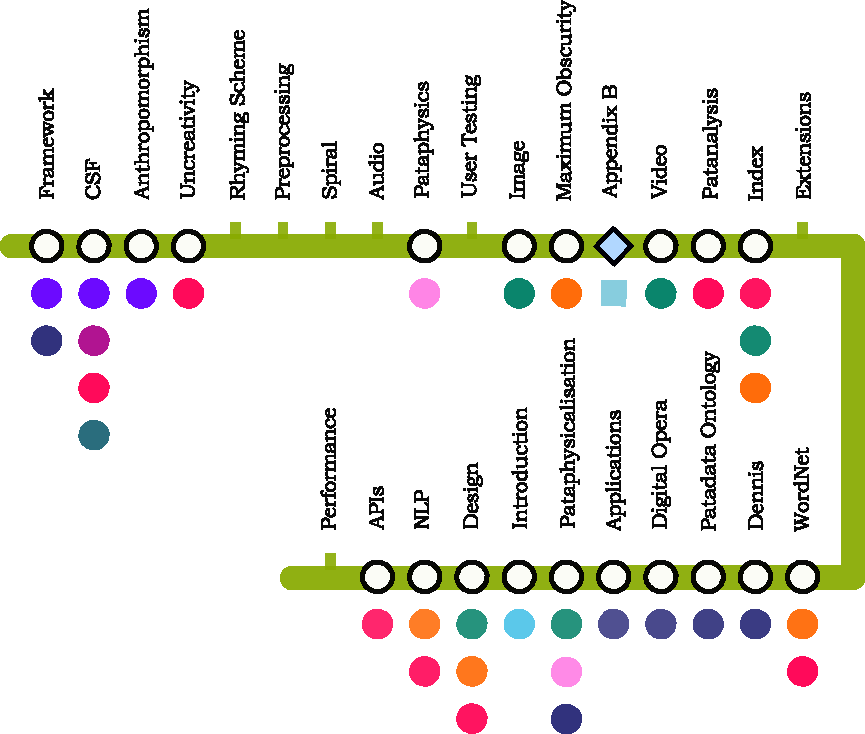
\includegraphics{aspi.pdf}
\end{figure}



\begin{figure}[!htb]
\centering
  
\includegraphics[width=\textwidth]{legend.pdf}
\end{figure}

\stopcontents[chapters]
